% AUTO-GENERATED by code/figlib.py helpers -- do not edit
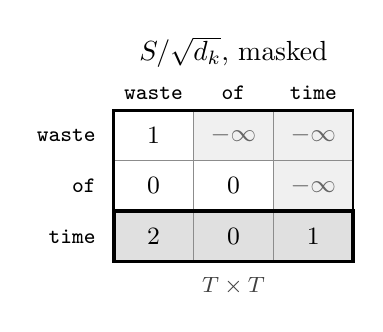
\begin{tikzpicture}[x=1.3cm]
\draw[black!45, fill=white] (0.000,0.000) rectangle (0.780,-0.640);
\node[font=\small, text=black] at (0.390,-0.320) {$1$};
\draw[black!45, fill=black!6] (0.780,0.000) rectangle (1.560,-0.640);
\node[font=\small, text=black!60] at (1.170,-0.320) {$-\infty$};
\draw[black!45, fill=black!6] (1.560,0.000) rectangle (2.340,-0.640);
\node[font=\small, text=black!60] at (1.950,-0.320) {$-\infty$};
\draw[black!45, fill=white] (0.000,-0.640) rectangle (0.780,-1.279);
\node[font=\small, text=black] at (0.390,-0.959) {$0$};
\draw[black!45, fill=white] (0.780,-0.640) rectangle (1.560,-1.279);
\node[font=\small, text=black] at (1.170,-0.959) {$0$};
\draw[black!45, fill=black!6] (1.560,-0.640) rectangle (2.340,-1.279);
\node[font=\small, text=black!60] at (1.950,-0.959) {$-\infty$};
\draw[black!45, fill=black!12] (0.000,-1.279) rectangle (0.780,-1.919);
\node[font=\small, text=black] at (0.390,-1.599) {$2$};
\draw[black!45, fill=black!12] (0.780,-1.279) rectangle (1.560,-1.919);
\node[font=\small, text=black] at (1.170,-1.599) {$0$};
\draw[black!45, fill=black!12] (1.560,-1.279) rectangle (2.340,-1.919);
\node[font=\small, text=black] at (1.950,-1.599) {$1$};
\draw[line width=1.4pt] (0.000,-1.279) rectangle (2.340,-1.919);
\draw[line width=0.9pt] (0.000,0.000) rectangle (2.340,-1.919);
\node[anchor=east, font=\footnotesize\ttfamily] at (-0.080,-0.320) {waste};
\node[anchor=east, font=\footnotesize\ttfamily] at (-0.080,-0.959) {of};
\node[anchor=east, font=\footnotesize\ttfamily] at (-0.080,-1.599) {time};
\node[anchor=south, font=\footnotesize\ttfamily] at (0.390,0.020) {waste};
\node[anchor=south, font=\footnotesize\ttfamily] at (1.170,0.020) {of};
\node[anchor=south, font=\footnotesize\ttfamily] at (1.950,0.020) {time};
\node[anchor=south, font=\normalsize] at (1.170,0.420) {$S/\sqrt{d_k}$, masked};
\node[anchor=north, font=\footnotesize, text=black!75] at (1.170,-1.999) {$T\times T$};
\end{tikzpicture}
